\chapter{The Thick--Client Software--System Architecture of \yerotherpblack}

\vspace{-2em}

\YEROTHCHAPINTRO{
This chapter explains why \yerotherpblack is modular
in its uses, and fits any industrial setting !
}

\vspace{1em}

\section{Business and user interface code deployment}

Table~\ref{tab:thickclient-application-againts-webbrowserbased-application}
depicts the issue of business and user
interface code deployment on all computers
participating in the functioning of \yerotherpblack,
as a software--system for a user.

We tackle the problem of automatic deployment of
business and user interface code on all user
computers by using the '\texttt{apt upgrade}'
software--system on '\debianlinux'.


\section{Sample technical configurations}

This section illustrates $2$ different possible
technical computer network configurations that
could prevail in the industry. 

\newpage

\subsection{Sample $2$--computers store}

\begin{center}
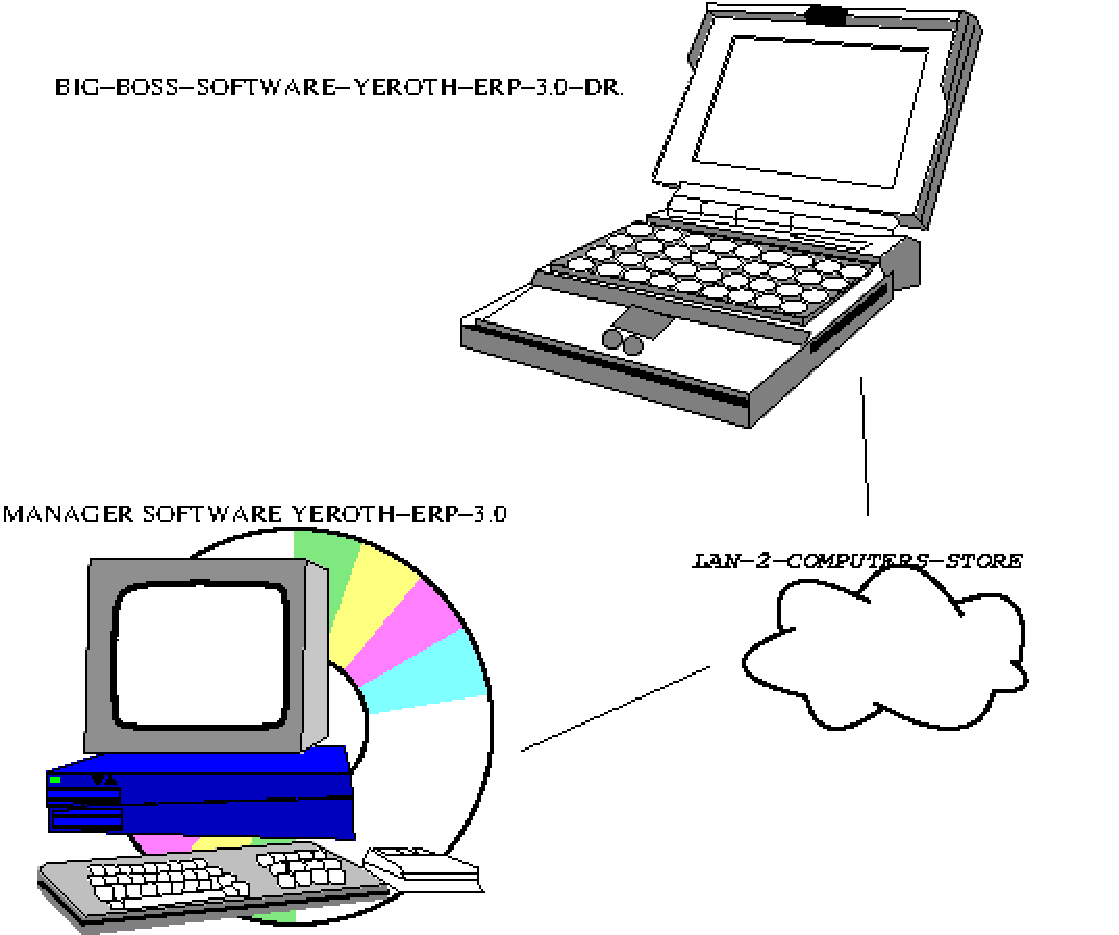
\includegraphics[scale=0.7]{images/yeroth-erp-sample-2-computers-store.pdf}
\captionof{figure}{Sample $2$--computers store.}
\label{fig:sample-two-computers-store}
\end{center}
\index{Sample $2$--computers store}

\newpage

\subsection{Sample decentralized multi sites supermarket}

\begin{center}
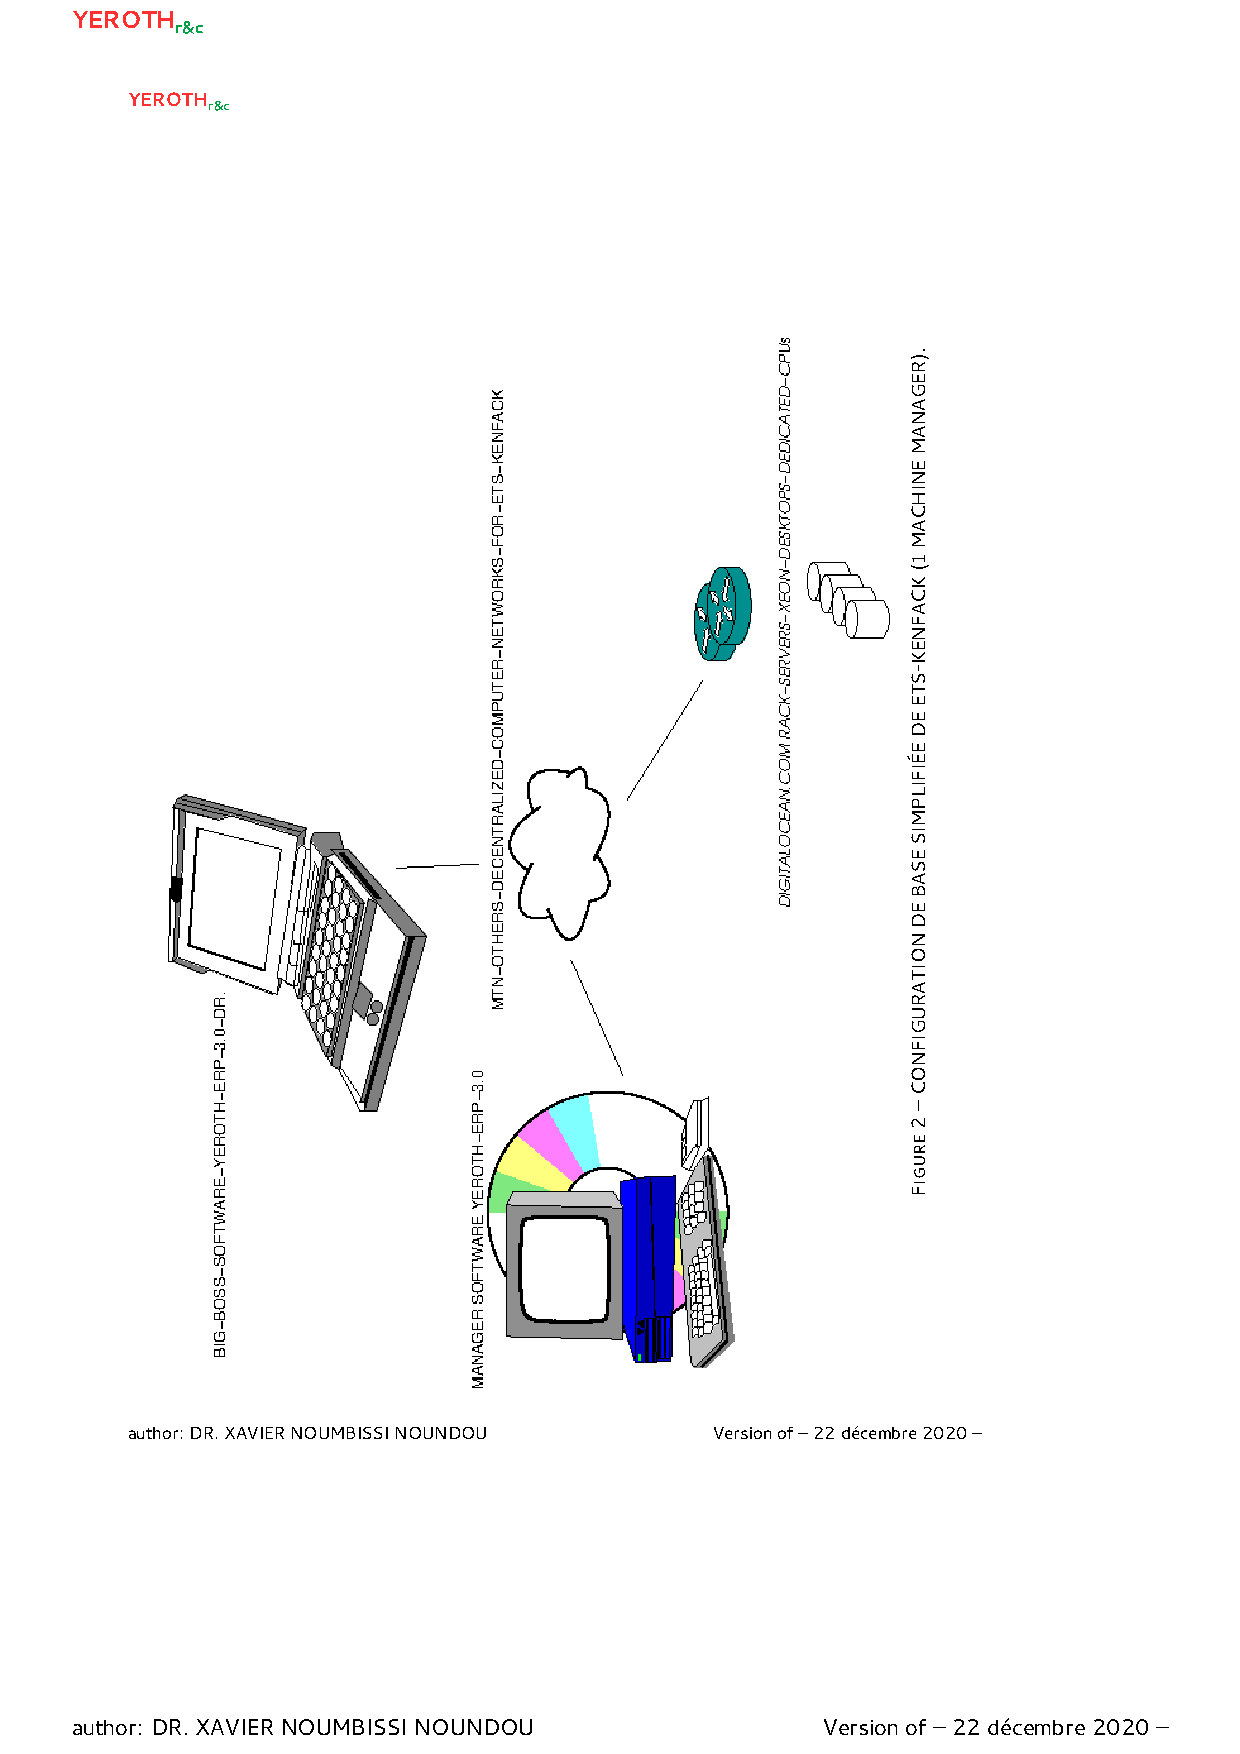
\includegraphics[scale=0.81]{images/yeroth-sample-decentralized-multi-sites-supermarket.pdf}
\captionof{figure}{Sample decentralized multi sites supermarket.}
\label{fig:sample-decentralized-multi-sites-supermarket}
\end{center}
\index{sample decentralized multi sites supermarket}